\subsection{POTENTIAL VALUE WITH INTERNAL OPPORTUNITIES.} 


The equity valuation of \textcolor{principal}{\empresaSolicitante} was conducted based on the business and financial information provided by the applicant, applying the theoretical framework of business valuation; under point 3 of the McKinsey Pentagon (\textit{``Value with internal improvements''}): (\textcolor{terciario}{\autoref{fig:hexagono}}).

\begin{figure}[H]
\centering
\caption{Opportunity Exploitation Pentagon \label{fig:hexagono}}\vspace{10pt}
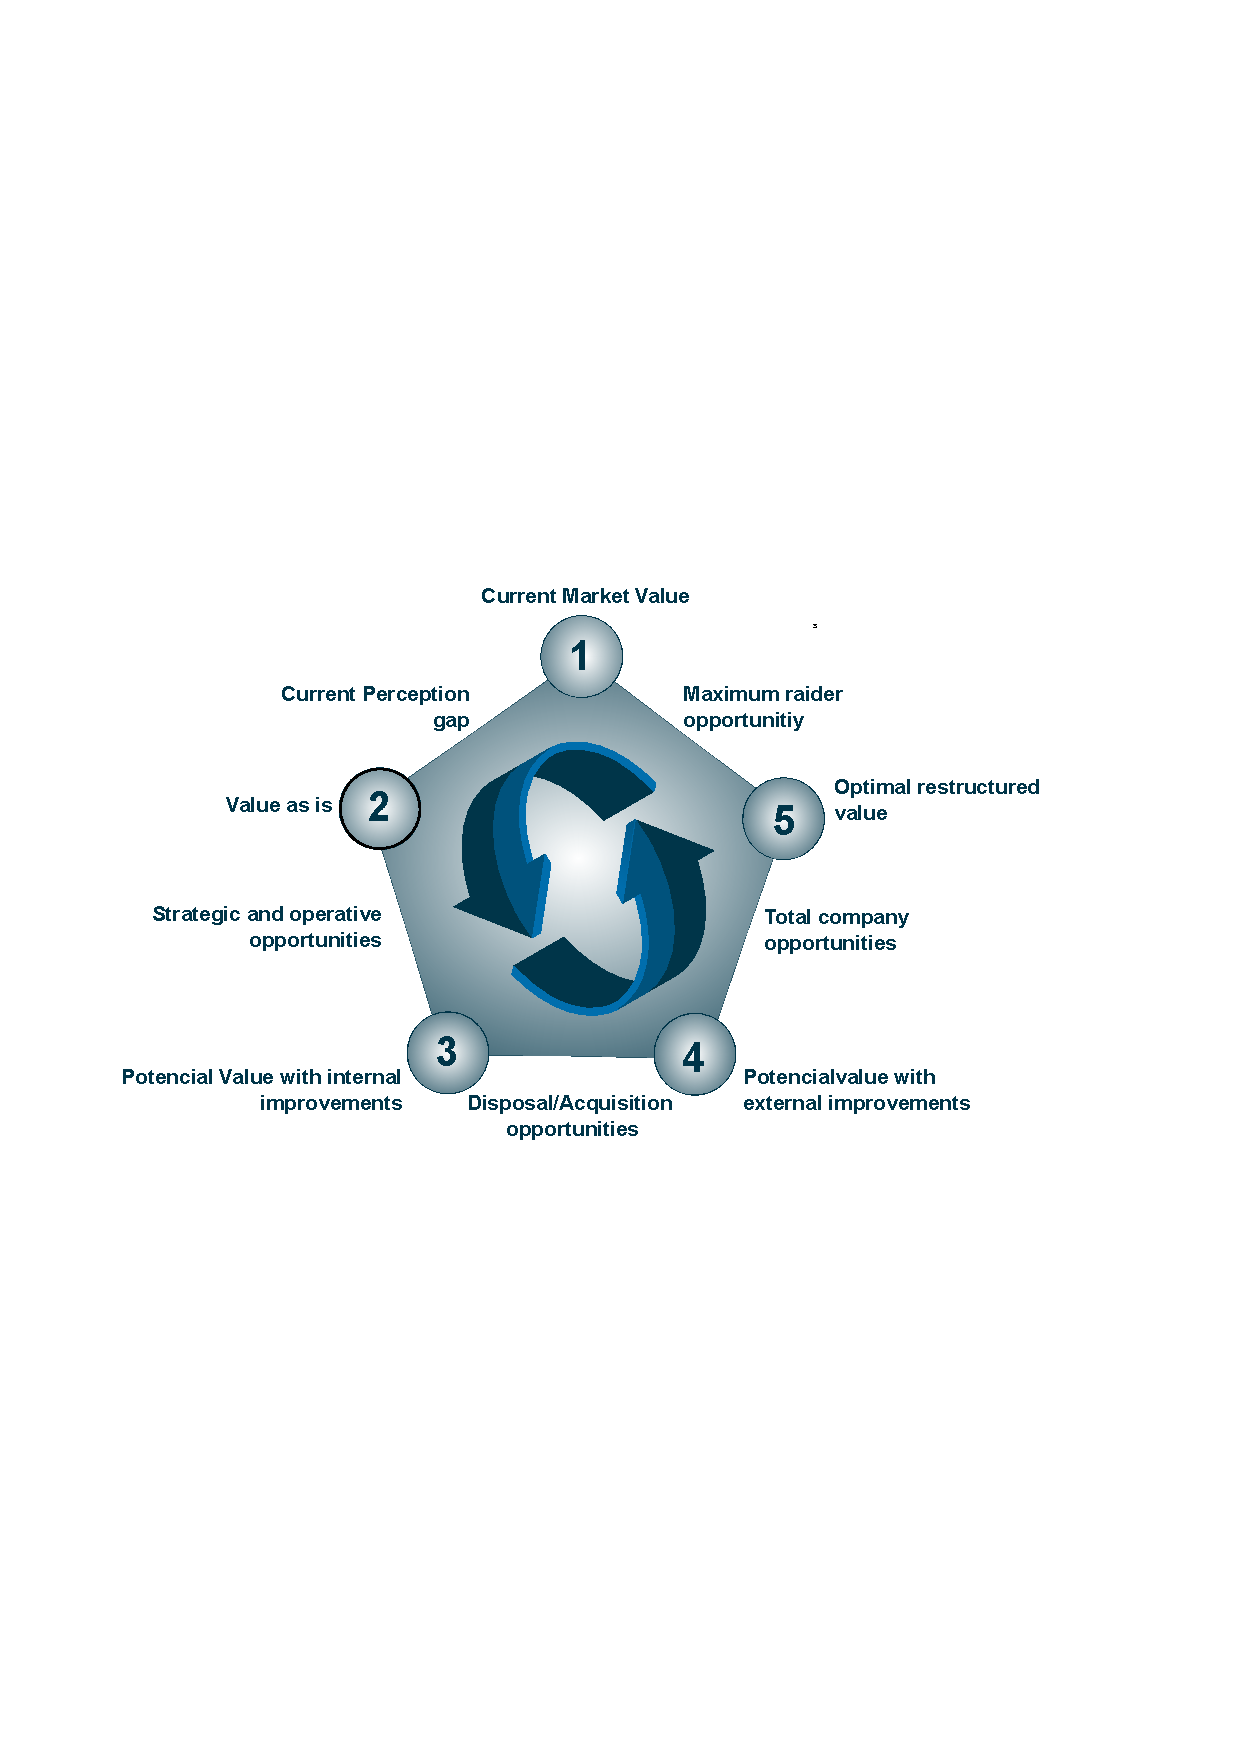
\includegraphics[width=8cm]{\rutaImagenes/penthagon}\\
Source: Valuation. Copeland Tom, Koller Tim y Murrin Jack.\\

John Wiley \& Sons. 2000.
\end{figure}

``\textcolor{secundario}{Value with internal improvements}.- It is the value acquired by the valued economic unit once the identification and exploitation of internal factors have been carried out. To achieve this, deficiencies are corrected, processes are improved and optimized, and new strategic opportunities are exploited, thus obtaining a higher value of the economic unit.''\\

